\documentclass[14pt,aspectratio=1610]{beamer}
%\documentclass[12pt,aspectratio=1610,handout]{beamer}
\usepackage{csu-theme}

\title{\Huge{} Quadtrees}
\subtitle{CSCI 315: Data Structure Analysis}
\author{Sean T. Hayes, Ph.D.}
\institute{Charleston Southern University}

%% Comment out date to use default (today)
% \date{April 15, 2025}
\subject{Software Programming}
%\keywords{}

\setlength{\parskip}{0.5em}

\usepackage{tikz}

\tikzset{
  point/.style={
    circle,
    fill=white,
    draw=white,
    very thick,
    minimum size=8pt,
    inner sep=0pt,
  }
}

% Used for 3D Plot of Quadtree
\usepackage{pgfplots}
\pgfplotsset{compat=newest}

\begin{document}

\begin{frame}
  \titlepage{}
\end{frame}

\section*{Motivation}

\begin{frame}{Outline}
\begin{itemize}[<+->]
  \item
    Motivation
  \item
    Explanation
  \item
    Time Complexity
  \item
    Implementation
  \item
    Variations of the Quadtree
\end{itemize}
\end{frame}

\begin{frame}{Motivation}
\begin{minipage}[t][2em][c]{\textwidth}
  \alt<-3>{
    Suppose we have a set of 2D points and we want to \\
    be able to query how many points lie in a particular rectangle.
  }{
    \alt<-4>{
      A brute force approach would be $O(n)$ in the number of points.\\
    }{
      We want a way to more efficiently count points\\ contained within a rectangular region.
    }
  }
\end{minipage}
\center
\begin{tikzpicture}[scale=0.50]
  \onslide<2->{
    \draw[very thick, fill=CSUcyan, draw=CSUgold] (12, 6) rectangle (20, 9);
  }
  \foreach \position in {
    (5.1, 8.3),
    (12.2, 2.9),
    (17.1, 6.1),
    (19.0, 5.7),
    (19.9, 1.1),
    (.7, 6.0),
    (7.2, 9.8),
    (11.9, 1.9),
    (16.3, 1.4),
    (10.7, 1.6),
    (17.2, 4.8),
    (10.2, 7.8),
    (1.9, 5.9),
    (.9, 3.1),
    (18.1, .3),
    (10.1, 8.4),
    (16.3, 7.0),
    (12.7, 5.0),
    (11.0, .1),
    (4.4, 6.2),
    (14.9, 8.9),
    (19.6, 1.5),
    (13.7, 5.1),
    (15.9, 9.4),
    (9.7, 2.6),
    (14.4, 3.8),
    (3.2, .2),
    (.9, 2.9),
    (14.8, 2.5),
    (6.1, 9.8),
    (12.1, .9),
    (11.1, .4),
    (16.6, .8),
    (13.2, 9.5),
    (8.7, 7.9),
    (18.2, 4.1),
    (10.7, 7.2),
    (2.0, 5.9),
    (1.9, 4.3),
    (11.1, 4.9),
    (12.7, .0),
    (15.1, 7.6),
    (4.4, .2),
    (.1, 2.8),
    (18.8, .6),
    (10.8, 7.7),
    (18.3, 2.7),
    (4.3, 6.2),
    (18.5, 7.2),
    (17.2, 1.6),
    (19.2, 1.0),
    (9.5, 5.2),
    (1.5, 5.7),
    (19.6, 5.6),
    (15.4, 1.8),
    (4.5, 5.5),
    (9.3, .9),
    (10.1, 2.0),
    (10.9, 6.4),
    (12.0, 9.1),
    (8.9, 7.4),
    (10.0, 7.3),
    (17.1, 5.3),
    (3.5, 3.3),
    (1.1, .2),
    (4.1, 9.0),
    (15.0, 1.7),
    (16.4, 9.6),
    (5.5, .8),
    (7.0, 5.4),
    (13.0, 7.8)
  }
    \node[point] at \position {};

\end{tikzpicture}
\onslide<5>{}
\end{frame}

\section {Explanation}
\begin{frame}{Explanation}
\begin{minipage}[t][3em][c]{\textwidth}
\alt<-3>{
  Each node in a Quadtree has a bounding rectangle.\\
  If the node is not a leaf then it has 4 children, \\
  splitting the rectangle into four quadrants.
}{
  \alt<-5>{
    Points are also attached to nodes.\\
    We define a constant specifying the maximum number of points associated with each node.
    }{
      Once that limit is exceeded, the node is subdivided into four quadrants.
    }
}
\end{minipage}

\centering
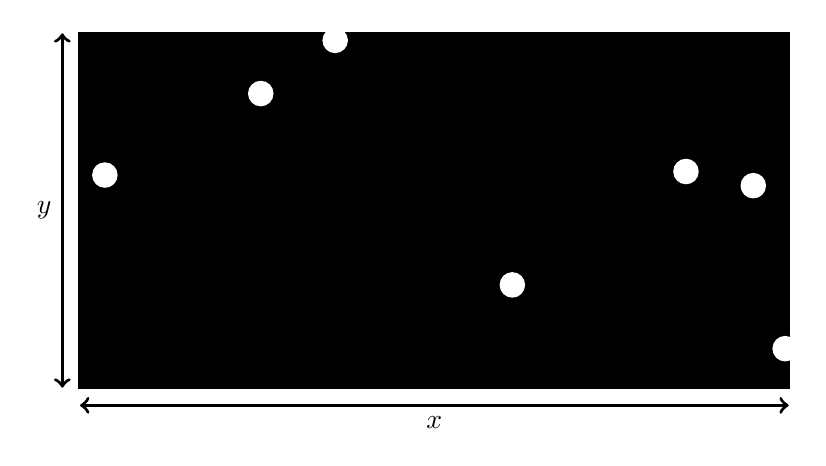
\begin{tikzpicture}[scale=0.45]
  
  \onslide<2->{
    \draw[very thick, fill=black] (0, 0) rectangle (20, 10);
    %\draw[very thick] (0, 0) rectangle (20, 10);
    \draw[<->, very thick] (0, -0.5) -- (20, -0.5) node [midway, below] {$x$};
    \draw[<->, very thick] (-0.5, 0) -- (-0.5, 10) node [midway, left] {$y$};
  }
  \onslide<3->{
    \draw[very thick, dotted] (0, 5) -- (20, 5);
    \draw[very thick, dotted] (10, 0) -- (10, 10);
  }

  \onslide<5->{
    \foreach \position in {
      (5.1, 8.3),
      (12.2, 2.9),
      (17.1, 6.1),
      (19.0, 5.7),
      (19.9, 1.1),
      (.7, 6.0),
      (7.2, 9.8)%,
      % (11.9, 1.9),
      % (16.3, 1.4),
      % (10.7, 1.6),
      % (17.2, 4.8),
      % (10.2, 7.8),
      % (1.9, 5.9),
      % (.9, 3.1),
      % (18.1, .3),
    }
    \node[point] at \position {};
  }
\end{tikzpicture}
\end{frame}

\begin{frame}{Insertion}
\begin{minipage}[t][3em][c]{0.8\textwidth}
\alt<-6>{
  Consider how points are inserted into a Quadtree
  that limits each node to have at most 5 points.
}{%
  \alt<-7>{%
    The root node is full, so the next point that is
    inserted will be placed on a child node.
  }{%
    \alt<-9>{%
      The bounding region is split up into four equal
      parts at this point and 4 children are created.
    }{
      \alt<-20>{%
        Any newly inserted points will be passed along
        to the children since the root node is ``full.''
      }{%
        Now the southeast child of the root has also reached
        the 5-point limit, so the node will also subdivide
        once a new point is added to it.
      }
    }
  }
}
\end{minipage}

\centering
\begin{tikzpicture}[scale=0.45]
  \draw[very thick, fill=black] (0, 0) rectangle (20, 10);
  \draw[<->, very thick] (0, -0.5) -- (20, -0.5) node [midway, below] {$x$};
  \draw[<->, very thick] (-0.5, 0) -- (-0.5, 10) node [midway, left] {$y$};

  \onslide<9->{
    \draw[line width=2.5pt, draw=yellow!80!black] ([xshift=3pt, yshift=3pt]0, 5) rectangle ([xshift=-3pt, yshift=-3pt]10, 10);
    \draw[line width=2.5pt, draw=codeKeyword] ([xshift=3pt, yshift=3pt]10, 5) rectangle ([xshift=-3pt, yshift=-3pt]20, 10);

    \draw[line width=2.5pt, draw=green] ([xshift=3pt, yshift=3pt]0, 0) rectangle ([xshift=-3pt, yshift=-3pt]10, 5);
    \draw[line width=2.5pt, draw=red] ([xshift=3pt, yshift=3pt]10, 0) rectangle ([xshift=-3pt, yshift=-3pt]20, 5);


    \only<23->{
      \draw[line width=2pt, draw=yellow!50!black] ([xshift=8pt, yshift=3pt]10, 2.5) rectangle ([xshift=-3pt, yshift=-8pt]15, 5);
      \draw[line width=2.5pt, draw=codeKeyword!50!black] ([xshift=3pt, yshift=3pt]15, 2.5) rectangle ([xshift=-8pt, yshift=-8pt]20, 5);

      \draw[line width=2pt, draw=green!50!black] ([xshift=8pt, yshift=8pt]10, 0) rectangle ([xshift=-3pt, yshift=-3pt]15, 2.5);
      \draw[line width=2.5pt, draw=red!50!black] ([xshift=3pt, yshift=8pt]15, 0) rectangle ([xshift=-8pt, yshift=-3pt]20, 2.5);
    }
  }

  \onslide<8->{
    \draw[very thick, dotted] (0, 5) -- (20, 5);
    \draw[very thick, dotted] (10, 0) -- (10, 10);

    \only<22-> {
      \draw[very thick, dotted] (10, 2.5) -- (20, 2.5);
      \draw[very thick, dotted] (15, 0) -- (15, 5);
    }
  }

  \only<2->{
    \node[point, fill=white] at (5.1, 8.3) {};
  }
  \only<3->{
    \node[point, fill=white] at (12.2, 2.9) {};
  }
  \only<4->{
    \node[point, fill=white] at (17.1, 6.1) {};
  }
  \only<5->{
    \node[point, fill=white] at (19.0, 5.7) {};
  }
  \onslide<6->{
    \node[point, fill=white] at (19.9, 1.1) {};
  }
  \onslide<11->{
    \node[point, fill=yellow!80!black] at (.7, 6.0) {};
  }
  \onslide<12->{
    \node[point, fill=yellow!80!black] at (7.2, 9.8) {};
  }
  \onslide<13->{
    \node[point, fill=red] at (11.9, 1.9) {};
  }
  \onslide<14->{
    \node[point, fill=red] at (16.3, 1.4) {};
  }
  \onslide<15->{
    \node[point, fill=red] at (10.7, 1.6) {};
  }
  \onslide<16->{
    \node[point, fill=red] at (17.2, 4.8) {};
  }
  \onslide<17->{
    \node[point, fill=codeKeyword] at (10.2, 7.8) {};
  }
  \onslide<18->{
    \node[point, fill=yellow!80!black] at (1.9, 5.9) {};
  }
  \onslide<19->{
    \node[point, fill=green] at (.9, 3.1) {};
  }
  \onslide<20->{
    \node[point, fill=red] at (18.1, .3) {};
  }


  \onslide<24->{
    \node[point, fill=green!50!black] at (11.0, .1) {};
  }
\end{tikzpicture}
\end{frame}

\begin{frame}{Query}
\begin{minipage}[t][3em][c]{\textwidth}
\begin{itemize}
  \item
    Use recursion to count the number of points in a\\given range.
  \item
    Consider only nodes that overlap with the query range.
\end{itemize}
\end{minipage}

\centering
\begin{tikzpicture}[scale=0.45]
  \draw[very thick, fill=black] (0, 0) rectangle (20, 10);
  \draw[<->, very thick] (0, -0.5) -- (20, -0.5) node [midway, below] {$x$};
  \draw[<->, very thick] (-0.5, 0) -- (-0.5, 10) node [midway, left] {$y$};

  \draw[fill=CSUcyan] (12, -0.25) rectangle (20.2, 7);

  %\onslide<9->{
    \draw[line width=2.5pt, draw=yellow] ([xshift=3pt, yshift=3pt]0, 5) rectangle ([xshift=-3pt, yshift=-3pt]10, 10);
    \draw[line width=2.5pt, draw=codeKeyword] ([xshift=3pt, yshift=3pt]10, 5) rectangle ([xshift=-3pt, yshift=-3pt]20, 10);

    \draw[line width=2.5pt, draw=green] ([xshift=3pt, yshift=3pt]0, 0) rectangle ([xshift=-3pt, yshift=-3pt]10, 5);
    \draw[line width=2.5pt, draw=red] ([xshift=3pt, yshift=3pt]10, 0) rectangle ([xshift=-3pt, yshift=-3pt]20, 5);


    %\only<23->{
      \draw[line width=2pt, draw=yellow!50!black] ([xshift=8pt, yshift=3pt]10, 2.5) rectangle ([xshift=-3pt, yshift=-8pt]15, 5);
      \draw[line width=2.5pt, draw=codeKeyword!50!black] ([xshift=3pt, yshift=3pt]15, 2.5) rectangle ([xshift=-8pt, yshift=-8pt]20, 5);

      \draw[line width=2pt, draw=green!50!black] ([xshift=8pt, yshift=8pt]10, 0) rectangle ([xshift=-3pt, yshift=-3pt]15, 2.5);
      \draw[line width=2.5pt, draw=red!50!black] ([xshift=3pt, yshift=8pt]15, 0) rectangle ([xshift=-8pt, yshift=-3pt]20, 2.5);
   % }
  %}
  \draw[very thick] (12, -0.25) rectangle (20.2, 7);

  %\onslide<8->{
    \draw[very thick, dotted] (0, 5) -- (20, 5);
    \draw[very thick, dotted] (10, 0) -- (10, 10);

    %\only<22-> {
      \draw[very thick, dotted] (10, 2.5) -- (20, 2.5);
      \draw[very thick, dotted] (15, 0) -- (15, 5);
    %}
  %}

  %\only<2->{
    \node[point, fill=white] at (5.1, 8.3) {};
  %}
  %\only<3->{
    \node[point, fill=white] at (12.2, 2.9) {};
  %}
  %\only<4->{
    \node[point, fill=white] at (17.1, 6.1) {};
  %}
  %\only<5->{
    \node[point, fill=white] at (19.0, 5.7) {};
  %}
  %\onslide<6->{
    \node[point, fill=white] at (19.9, 1.1) {};
  %}
  %\onslide<11->{
    \node[point, fill=yellow] at (.7, 6.0) {};
  %}
  %\onslide<12->{
    \node[point, fill=yellow] at (7.2, 9.8) {};
  %}
  %\onslide<13->{
    \node[point, fill=red] at (11.9, 1.9) {};
  %}
  %\onslide<14->{
    \node[point, fill=red] at (16.3, 1.4) {};
  %}
  %\onslide<15->{
    \node[point, fill=red] at (10.7, 1.6) {};
  %}
  %\onslide<16->{
    \node[point, fill=red] at (17.2, 4.8) {};
  %}
  %\onslide<17->{
    \node[point, fill=codeKeyword] at (10.2, 7.8) {};
  %}
  %\onslide<18->{
    \node[point, fill=yellow] at (1.9, 5.9) {};
  %}
  %\onslide<19->{
    \node[point, fill=green] at (.9, 3.1) {};
  %}
  %\onslide<20->{
    \node[point, fill=red] at (18.1, .3) {};
  %}


  %\onslide<24->{
    \node[point, fill=green!50!black] at (11.0, .1) {};
  %}
\end{tikzpicture}
\end{frame}


\begin{frame}{3D Visualization}
  \center{}
  \begin{tikzpicture}[every mark/.append style={thick, scale=1.6, draw=CSUblue!80!white, transform shape}]
    \begin{axis}[
        view/el=22, % reduce the vertical elevation
        zlabel=Tree Level,
        domain=-1:1,
        enlarge z limits=0.0,
        surf,
        shader=flat,
        xtick distance=1,
        ytick distance=1,
        ztick distance=1,
        tickwidth=0,
        axis line style={white},
        text=white,
        xticklabel=\empty,
        yticklabel=\empty,
        z dir=reverse,
        very thick,
        line cap=round,
      ]

      % Level 2
      \addplot3[yellow!50!black, fill opacity=0.75] coordinates {
          (15, 5, 2) (10, 5, 2)
  
          (15, 2.5, 2) (10, 2.5, 2)
        };

      \addplot3[green!50!black, fill opacity=0.75] coordinates {
          (15, 2.5, 2) (10, 2.5, 2)
  
          (15, 0, 2) (10, 0, 2)
      };

      \addplot3[codeKeyword!50!black, fill opacity=0.75] coordinates {
          (20, 5, 2) (15, 5, 2)
  
          (20, 2.5, 2) (15, 2.5, 2)
        };

      \addplot3[red!50!black, fill opacity=0.75] coordinates {
          (20, 2.5, 2) (15, 2.5, 2)
  
          (20, 0, 2) (15, 0, 2)
        };

        
      
      % Level 1
      \addplot3[green, fill opacity=0.67] coordinates {
          (10, 5, 1) (0, 5, 1)
  
          (10, 0, 1) (0, 0, 1)
        };
      
      \addplot3[yellow, fill opacity=0.67] coordinates {
          (10, 10, 1) (0, 10, 1)
  
          (10, 5, 1) (0, 5, 1)
        };

      \addplot3[red, fill opacity=0.67] coordinates {
          (20, 5, 1) (10, 5, 1)
  
          (20, 0, 1) (10, 0, 1)
        };

      \addplot3[codeKeyword, fill opacity=0.67] coordinates {
          (20, 10, 1) (10, 10, 1)
  
          (20, 5, 1) (10, 5, 1)
        };

      % Root
      \addplot3[white, fill opacity=0.67] coordinates {
        (0, 0, 0) (20, 0, 0)

        (0, 10, 0) (20, 10, 0)
      };

      % Root
      \addplot3[only marks, white] coordinates {
          % (0, 0, 1)
          (5.1, 8.3, 0)
          (12.2, 2.9, 0)
          (17.1, 6.1, 0)
          (19.0, 5.7, 0)
          (19.9, 1.1, 0)
        };

      \addplot3[only marks, yellow!80!white] coordinates {
          (.7, 6.0, 1) % yellow
          (7.2, 9.8, 1) % yellow
          (1.9, 5.9, 1) % yellow
        };

      \addplot3[only marks, red!80!white] coordinates {
          (11.9, 1.9, 1) % red
          (16.3, 1.4, 1) % red
          (10.7, 1.6, 1) % red
          (17.2, 4.8, 1) % red
          (18.1, .3, 1) % red
        };

      \addplot3[only marks, green!80!white] coordinates {
          (.9, 3.1, 1) % green
        };

      \addplot3[only marks, codeKeyword] coordinates {
          (10.2, 7.8, 1) % codeKeyword
        };

      \addplot3[only marks, green!67!black, every mark/.append style={draw=CSUblue!20!white}] coordinates {
          (11.0, .1, 2) % dark green
        };


      
    \end{axis}
  \end{tikzpicture}
\end{frame}

\section{Time Complexity}

\begin{frame}{Time Complexity}
\begin{minipage}[t][3em][c]{\textwidth}
  \center
  If the points are distributed uniformly in the root's \\
  range, then insertions and queries are \emph{logarithmic}.
\end{minipage}
\center
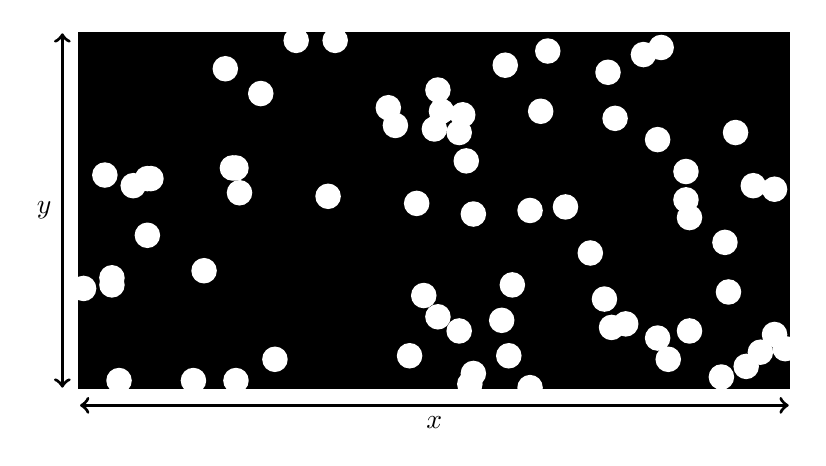
\begin{tikzpicture}[scale=0.45]
  \draw[very thick, fill=black] (0, 0) rectangle (20, 10);
  \draw[<->, very thick] (0, -0.5) -- (20, -0.5) node [midway, below] {$x$};
  \draw[<->, very thick] (-0.5, 0) -- (-0.5, 10) node [midway, left] {$y$};

  \foreach \position in {
    (5.1, 8.3),
    (12.2, 2.9),
    (17.1, 6.1),
    (19.0, 5.7),
    (19.9, 1.1),
    (.7, 6.0),
    (7.2, 9.8),
    (11.9, 1.9),
    (16.3, 1.4),
    (10.7, 1.6),
    (17.2, 4.8),
    (10.2, 7.8),
    (1.9, 5.9),
    (.9, 3.1),
    (18.1, .3),
    (10.1, 8.4),
    (16.3, 7.0),
    (12.7, 5.0),
    (11.0, .1),
    (4.4, 6.2),
    (14.9, 8.9),
    (19.6, 1.5),
    (13.7, 5.1),
    (15.9, 9.4),
    (9.7, 2.6),
    (14.4, 3.8),
    (3.2, .2),
    (.9, 2.9),
    (14.8, 2.5),
    (6.1, 9.8),
    (12.1, .9),
    (11.1, .4),
    (16.6, .8),
    (13.2, 9.5),
    (8.7, 7.9),
    (18.2, 4.1),
    (10.7, 7.2),
    (2.0, 5.9),
    (1.9, 4.3),
    (11.1, 4.9),
    (12.7, .0),
    (15.1, 7.6),
    (4.4, .2),
    (.1, 2.8),
    (18.8, .6),
    (10.8, 7.7),
    (18.3, 2.7),
    (4.3, 6.2),
    (18.5, 7.2),
    (17.2, 1.6),
    (19.2, 1.0),
    (9.5, 5.2),
    (1.5, 5.7),
    (19.6, 5.6),
    (15.4, 1.8),
    (4.5, 5.5),
    (9.3, .9),
    (10.1, 2.0),
    (10.9, 6.4),
    (12.0, 9.1),
    (8.9, 7.4),
    (10.0, 7.3),
    (17.1, 5.3),
    (3.5, 3.3),
    (1.1, .2),
    (4.1, 9.0),
    (15.0, 1.7),
    (16.4, 9.6),
    (5.5, .8),
    (7.0, 5.4),
    (13.0, 7.8)
  }
    \node[point] at \position {};

\end{tikzpicture}
\end{frame}


\begin{frame}{Time Complexity}
\begin{minipage}[t][3.05em][c]{\textwidth}
  \center%
  However, if they are not uniformly distributed\\
  then it can degrade to \emph{linear time}.
\end{minipage}
\center%
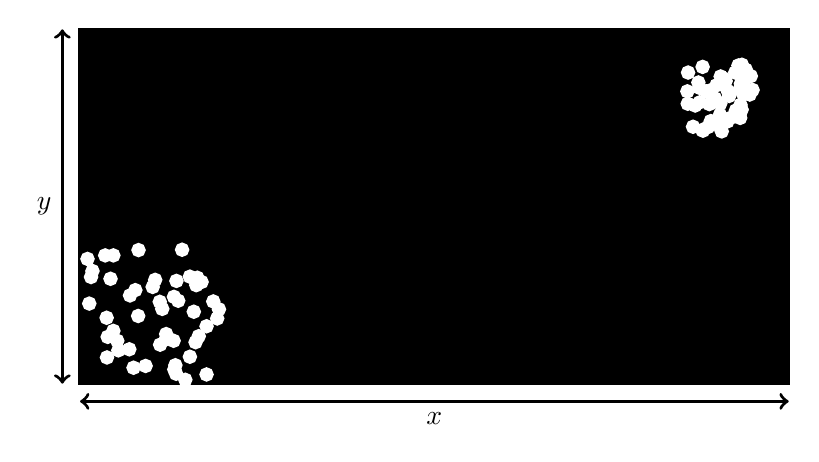
\begin{tikzpicture}[scale=0.45]
  \draw[very thick, fill=black] (0, 0) rectangle (20, 10);
  \draw[<->, very thick] (0, -0.5) -- (20, -0.5) node [midway, below] {$x$};
  \draw[<->, very thick] (-0.5, 0) -- (-0.5, 10) node [midway, left] {$y$};

  \foreach \position in {
    (2.42, 1.25),
    (3.31, 2.99),
    (2.43, 1.40),
    (3.35, 1.34),
    (3.21, 2.03),
    (1.05, 1.21),
    (2.66, .40),
    (2.97, .11),
    (.78, 1.32),
    (.71, 3.62),
    (3.28, 2.78),
    (3.57, .26),
    (2.26, 1.10),
    (1.85, .50),
    (3.76, 2.32),
    (2.88, 3.78),
    (3.92, 2.10),
    (.26, 2.26),
    (3.57, 1.62),
    (2.71, .28),
    (2.65, 2.45),
    (3.87, 1.84),
    (.94, 3.62),
    (.31, 3.01),
    (1.64, 1.91),
    (2.77, 2.34),
    (2.12, 2.93),
    (2.72, 2.90),
    (1.65, 3.77),
    (.75, 1.86),
    (3.43, 2.87),
    (.21, 3.52),
    (3.10, 3.02),
    (.94, 1.49),
    (1.41, 2.49),
    (1.51, .45),
    (1.08, .94),
    (.86, 2.96),
    (2.25, 2.31),
    (.35, 3.18),
    (2.32, 2.11),
    (2.05, 2.73),
    (3.26, 1.17),
    (.76, .74),
    (3.29, 2.86),
    (3.10, .76),
    (2.69, .52),
    (1.39, .97),
    (2.64, 1.21),
    (1.56, 2.64),
    (17.67, 8.25),
    (17.57, 8.94),
    (18.11, 7.12),
    (18.22, 8.54),
    (18.32, 8.12),
    (18.71, 8.41),
    (17.94, 7.33),
    (17.16, 8.78),
    (18.58, 8.98),
    (17.92, 8.05),
    (18.64, 7.87),
    (18.61, 7.56),
    (17.96, 8.42),
    (18.51, 7.71),
    (18.49, 8.78),
    (18.27, 7.40),
    (17.56, 7.16),
    (17.58, 7.14),
    (18.06, 7.59),
    (17.76, 7.89),
    (18.62, 8.31),
    (17.14, 8.25),
    (18.38, 7.51),
    (17.15, 7.90),
    (17.80, 7.41),
    (18.90, 8.16),
    (18.00, 7.44),
    (18.66, 7.75),
    (18.28, 8.26),
    (18.68, 9.00),
    (17.77, 8.27),
    (17.72, 7.24),
    (17.30, 7.25),
    (17.45, 8.50),
    (18.07, 7.91),
    (18.79, 8.86),
    (18.15, 8.62),
    (18.93, 8.68),
    (18.08, 8.67),
    (18.63, 7.50),
    (18.98, 8.29),
    (18.59, 7.74),
    (18.67, 7.73),
    (17.49, 7.94),
    (18.69, 8.25),
    (17.48, 8.35),
    (18.77, 8.60),
    (17.36, 7.85),
    (18.72, 8.16),
    (18.65, 8.47)
  }
    \node[point, minimum size=4pt] at \position {};

\end{tikzpicture}
\end{frame}

\section{Implementation}

\begin{frame}{Quadrant Contains a Point}
  
  \center{}
  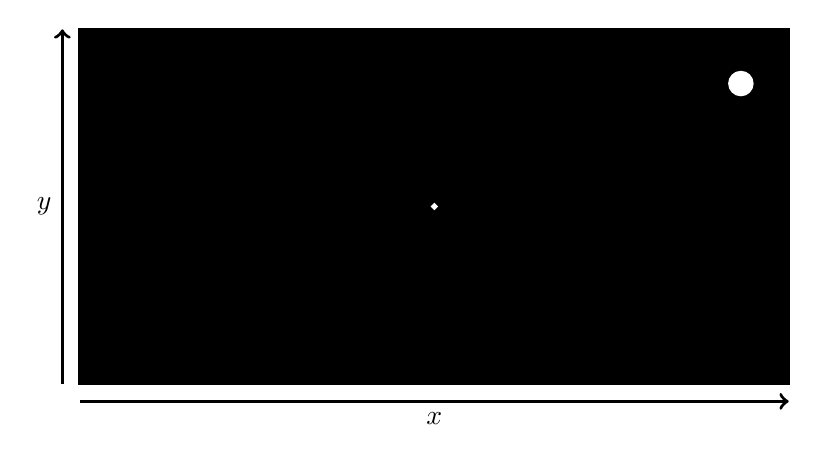
\begin{tikzpicture}[scale=0.45]
    \draw[very thick, fill=black] (0, 0) rectangle (20, 10);
    \draw[very thick, dotted] (0, 5) -- (10, 5);
    \draw[very thick, dotted] (10, 0) -- (10, 5);

    \draw[arrows={->}, very thick] (0, -0.5) -- (20, -0.5) node [midway, below] {$x$};
    \draw[arrows={->}, very thick] (-0.5, 0) -- (-0.5, 10) node [midway, left] {$y$};
    
    % \draw[->, very thick] (9.5, 5) -- (9.5, 0) node [midway, left] {\textit{center} $+$ \textit{half height}};

    % \node[point, fill=CSUcyan] at (10, 10) {};
    % \node[, anchor=north west, inner sep=3pt] at (10, 10) {$(c_x - \frac{1}{2}h, c_y)$};

    % \node[point, fill=CSUcyan] at (10, 0) {};
    % \node[, anchor=south west, inner sep=3pt] at (10, 0) {$(c_x + \frac{1}{2}h, c_y)$};

    % \node[point, fill=CSUcyan] at (0, 5) {};
    % \node[, anchor=north west, inner sep=3pt] at (0, 5) {$(c_x, c_y - \frac{1}{2}w)$};

    % \node[point, fill=CSUcyan] at (20, 5) {};
    % \node[, anchor=north east, inner sep=3pt] at (20, 5) {$(c_x, c_y + \frac{1}{2}w)$};
    

    \draw[arrows={stealth-stealth}, very thick, shorten >=1pt] (10, 5) -- (10, 10) node [midway, left] {$\frac{1}{2}h$};
    \draw[arrows={stealth-stealth}, very thick, shorten >=1pt] (10, 5) -- (20, 5) node [midway, below] {$\frac{1}{2}w$};

    % Center point and label
    \node[point, minimum size=1pt] at (10, 5) {};
    \node[, anchor=north east, inner sep=3pt] at (10, 5) {$(c_x, c_y)$};

    \node[point] at (18.65, 8.47) {};
    \node[, anchor=north east, inner sep=3pt] at (18.65, 8.47) {$(p_x, p_y)$};
  
  \end{tikzpicture}

  \((c_x - \frac{1}{2}w) \le p_x < (c_x + \frac{1}{2}w)\)

  \((c_y - \frac{1}{2}h) \le p_y < (c_y + \frac{1}{2}h)\)
\end{frame}

\begin{frame}{Region Intersects a Quad}
\begin{columns}
  \column{0.45\textwidth}
    \center{}
    \begin{tikzpicture}[scale=0.55]
      \draw[draw=none, fill=CSUcyan!20!black] (3.5, 2.5) rectangle (7.5, 5.5);
      \draw[draw=none, fill=CSUgold!20!black] (-3.5, -2.5) rectangle (0.5, 0.5);
      \draw[draw=none, fill=green!20!black] (-3.5, 2.5) rectangle (0.5, 5.5);
      \draw[draw=none, fill=yellow!20!black] (3.5, -2.5) rectangle (7.5, 0.5);

      \draw[draw=none, fill=black, opacity=0.5] (0, 0) rectangle (4, 3);
      
      \draw[draw=CSUcyan, very thick, fill=none] (3.5, 2.5) rectangle (7.5, 5.5);
      \draw[draw=CSUgold, very thick, fill=none] (-3.5, -2.5) rectangle (0.5, 0.5);
      \draw[draw=green, very thick, fill=none] (-3.5, 2.5) rectangle (0.5, 5.5);
      \draw[draw=yellow, very thick, fill=none] (3.5, -2.5) rectangle (7.5, 0.5);

      \draw[very thick, fill=none] (0, 0) rectangle (4, 3);
    
      \draw[->, very thick] (-4.0, -3) -- (7.5, -3) node [midway, below] {$x$};
      \draw[->, very thick] (-4, -3) -- (-4, 5.5) node [midway, left] {$y$};
    \end{tikzpicture}

  \column{0.3\textwidth}
    \center
    \begin{align*}
      \text{left} &< c_x + \frac{1}{2}w\\[5pt]
      \text{right} &> c_x - \frac{1}{2}w\\[5pt]
      \text{top} &> c_y - \frac{1}{2}h\\[5pt]
      \text{bottom} &< c_y + \frac{1}{2}h\\
    \end{align*} 
\end{columns}
\end{frame}

\section{Variations}

\begin{frame}{Types of Quadtrees}
  \begin{itemize}[<+->]
    \item
      \emph{Region} quadtree -- Divides region into sub-quadrants based on the areas with more detailed information.
      \begin{itemize}
        \item Image processing -- only subdivide if pixels differ in color.
        \item Variable resolution data field -- each parent has the average value of its children.
      \end{itemize}
    \item
      \emph{Point} quadtree -- Divide the region at the point that is inserted (like a binary tree but with 4 pointers). \href{https://en.wikipedia.org/wiki/K-d_tree}{$k$-d trees} are preferred.
    \item
      \emph{Point-region (PR)} quadtree -- What we implemented.
    \item
      \emph{Edge} quadtree -- Stores lines/curves with approximation.
    \item
      \emph{Polygonal map (PM)} quadtree -- stores polygons.
    \item
      \emph{Compressed} quadtrees -- only storing subtrees whose leaves have interesting data and removing empty intermediate nodes.
  \end{itemize}
\end{frame}

\begin{frame}{Conclusion}
\begin{itemize}
  \item
    Quadtrees are used to efficiently query the number of points contained within various rectangular ranges.
  \item
    Quadtrees are most efficient when the points are uniformly distributed.
\end{itemize}
\end{frame}


% \begin{frame}{Intersection}
% \center
% \begin{tikzpicture}[scale=0.45]
%   \draw[very thick, fill=black] (0, 0) rectangle (20, 10);
%   \draw[<->, very thick] (0, -0.5) -- (20, -0.5) node [midway, below] {$x$};
%   \draw[<->, very thick] (-0.5, 0) -- (-0.5, 10) node [midway, left] {$y$};

%   \draw[very thick, dotted] (0, 5) -- (20, 5);
%   \draw[very thick, dotted] (10, 0) -- (10, 10);
% \end{tikzpicture}
% \end{frame}

\section*{Lab 24}
\begin{frame}{Lab 24: Quadtrees}
\begin{center}\Large
Let's take a look at the lab based on today's lecture.
\end{center}
\end{frame}
\end{document}